\chapter{Office 和 WPS——办公样样行}
\label{office-and-wps}

\begin{note}
  欢迎来到《Missing》软件篇!在基础篇我们介绍了最最基本的电脑操作,例如文件管理和软件安装。
  而在软件篇中,我们会「介绍」一些软件。
  这里的「介绍」并不是教你怎么用这个软件,而是简要说明这个软件是干什么的、有什么特点,以及为什么我们会介绍它。
  请注意,《Missing》从来不是任何软件使用教程的替代品。
\end{note}

\begin{intro}
  让我们从最常见的办公软件——Office,和它的相似物 WPS,来开始我们的软件篇旅程。
  在阅读完这一部分后,你能找到下面这些问题的答案:
  \begin{itemize}
    \item 下面五个名词之间的关系:Word、PowerPoint (简称 PPT)、Excel、Office、WPS。
    \item Office 版本好多,我该选哪个?2003?2007?2019?
    \item 为什么我电脑上自带的 Office 点开之后却打开了一个网页 / 购买链接?
    \item Office 怎么装?
    \item WPS 跟 Office 有什么区别?既然前者免费,那为什么还要后者?
  \end{itemize}
\end{intro}

我们绝大多数人使用电脑,都逃不开「文档写作」「幻灯片制作」「表格处理」这么三件事。
也许你早已会用 WPS,或者 Word、PPT 以及 Excel 这些再熟悉不过的软件来做这三件事,但这些软件背后的故事或许并不为你所知晓。

仍然首先强调,这部分并不是一份 Office 软件教程。

\section{Microsoft Office}

Microsoft Office 是由微软(也就是 Windows 系统它爹)开发的办公软件套装。
称它「软件套装」,是因为 Microsoft Office 是一系列软件的组合,而非一个单个的软件。
Microsoft Office 一般被人们直接简称为「Office」。
Office 包含了一系列面向办公领域的软件。
下面列出 Office 中的一些子软件:

\begin{itemize}
  \item \regcolor{Word,用于制作文稿。}
  \item \regcolor{PowerPoint(往往简称「PPT」),用于制作幻灯片。}
  \item \regcolor{Excel,用于制作表格和进行数据处理。}
  \item OneNote,用于记笔记。
  \item Access,用于制作和管理数据库。
  \item Publisher,用于编辑出版物(例如,成册的书籍排版)。
  \item Visio,用于绘制各种图案。
  \item ……
\end{itemize}

上面列表中的前三者,即 Word、PPT 和 Excel,是 Office 套装中人们耳熟能详的三个子应用,民间俗称「Office 三件套」。
它们三个能满足几乎所有的基本办公需求,而其他的 Office 子应用有些专业而复杂,使用的人相对不多,因而很多时候都没什么人安装。

最新版本的 Office 三件套的软件图标如下图所示。

\begin{figure}[htb!]
  \centering
  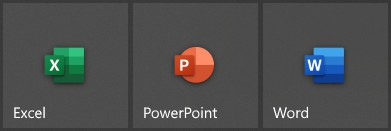
\includegraphics[width=6cm]{assets/Office_Icons.jpg}
  \caption{如今的 Office 图标}
  \label{Office_Icons}
\end{figure}

\subsection{Office 的历史与版本}

Office 是一款历史悠久的软件套装,它诞生于二十世纪八九十年代。
近 20 年,Office 都使用年份作为版本名称。

Office 2003 是十分经典的一代 Office。
与现在的 Office 软件界面有很大不同,Office 2003 的功能按钮是一排排地「罗列」在软件界面上方的。
下图是 Word 2003 的软件界面。

\begin{figure}[htb!]
  \centering
  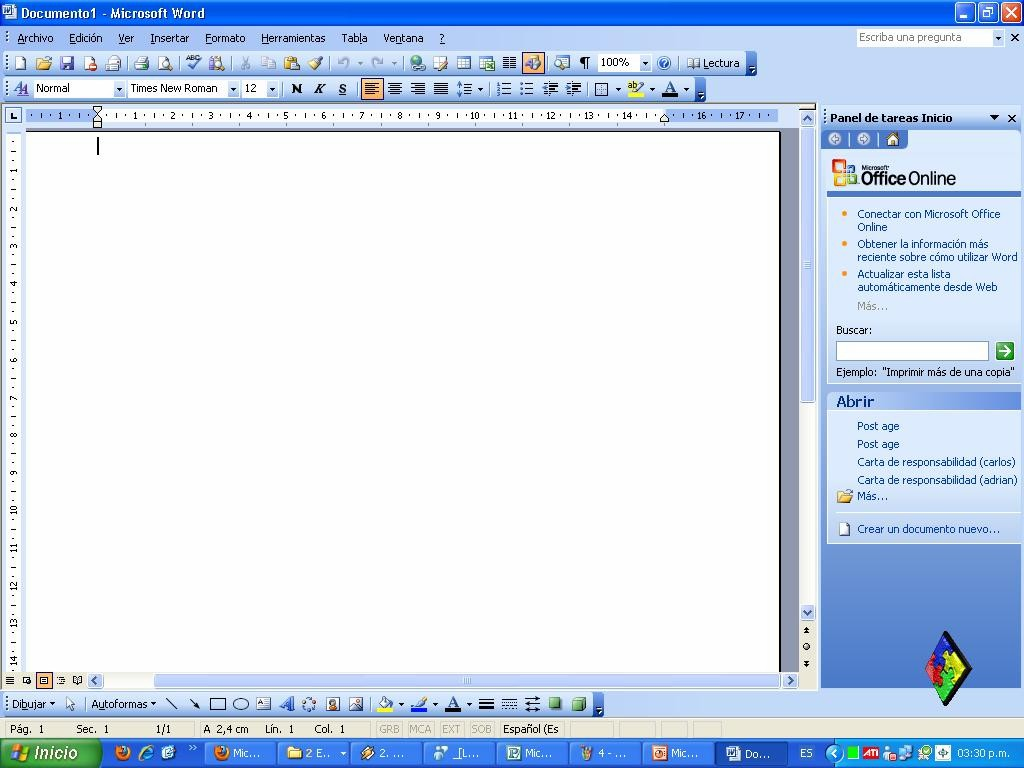
\includegraphics[width=11cm]{assets/Word_2003.jpg}
  \caption{Word 2003 的界面}
  \label{Word_2003}
\end{figure}

经典归经典,由于年代实在太过久远,在今天(2023 年),除了部分中小学的「信息技术」课堂外,我们几乎很少再见到这一版 Office。

Office 2007 同样是经典的一代 Office。
自 Office 2007 开始,Office 软件采用了一种新的用户界面——「Ribbon」。
直到今天,Office 的软件界面仍然有着 2007 版本的许多影子。
另一方面,这种新的界面与 2003 版及其之前的版本有着很大的不同。
出于这个原因,当时许多人不愿意迁移至新版本。
下图是 Word 2007 的软件界面。

\begin{figure}[htb!]
  \centering
  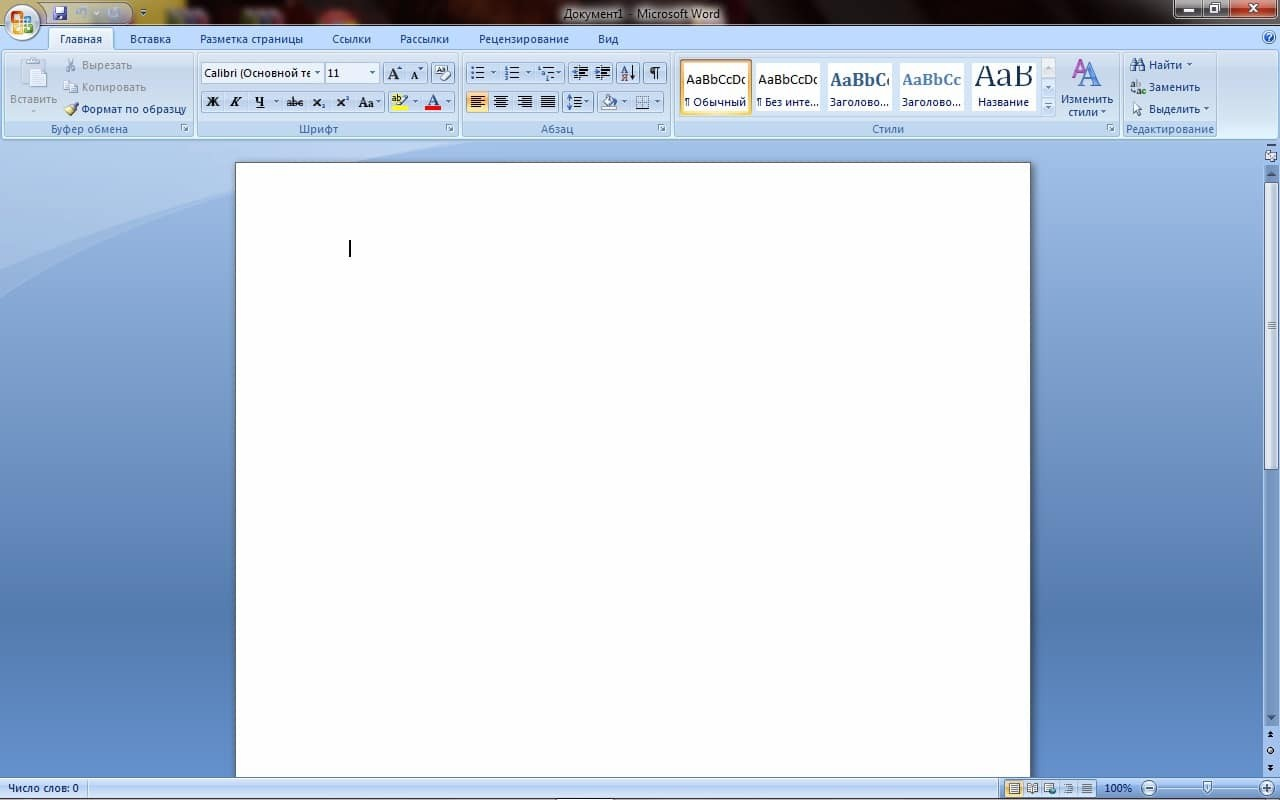
\includegraphics[width=11cm]{assets/Word_2007.jpg}
  \caption{Word 2007 的界面}
  \label{Word_2007}
\end{figure}

不难发现,Ribbon 界面的主要特点是:
功能按钮按照一定的分类分置于不同的「选项卡」中,在软件上方错落排开,与 Office 2003 那种按钮一排排罗列的操作方式大相径庭。

Office 2010 与 Office 2007 在软件界面和风格上并没有什么很大的差别。
在 2021 年以前,我国计算机二级考试 Office 科目使用的就是 Office 2010 版本,因而下面的 Word 2010 软件界面想必许多读者都不会陌生。

\begin{figure}[htb!]
  \centering
  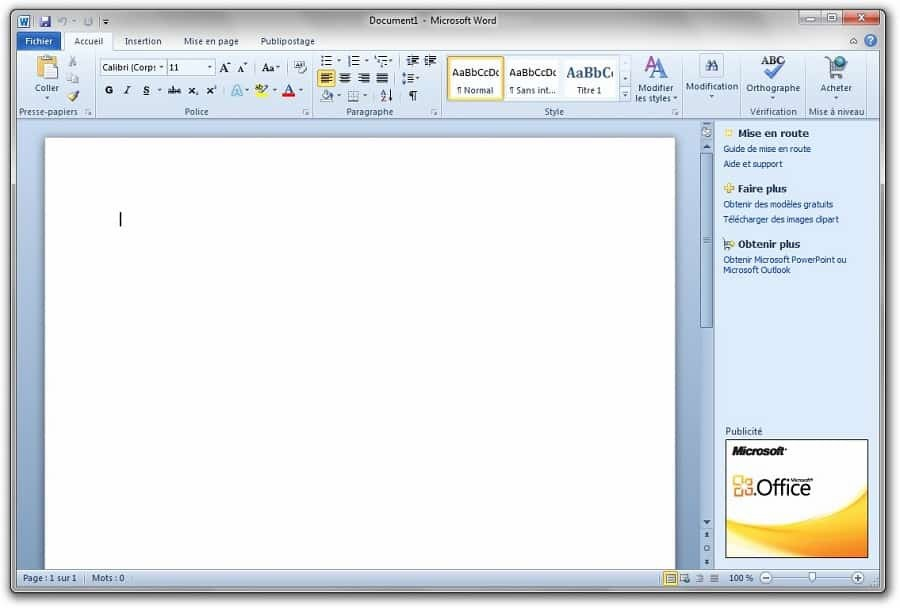
\includegraphics[width=11cm]{assets/Word_2010.jpg}
  \caption{Word 2010 的界面}
  \label{Word_2010}
\end{figure}

Office 2013 开始,Office 的界面画风从原来的「拟物」变成了「扁平」,不过操作逻辑仍然是自 Office 2007 就有的那一套。
Office 2013、2016、2019 乃至 2021 在界面上长得都差不多,操作体验也差不多。
下图是 Word 2019 的软件界面。

\begin{figure}[htb!]
  \centering
  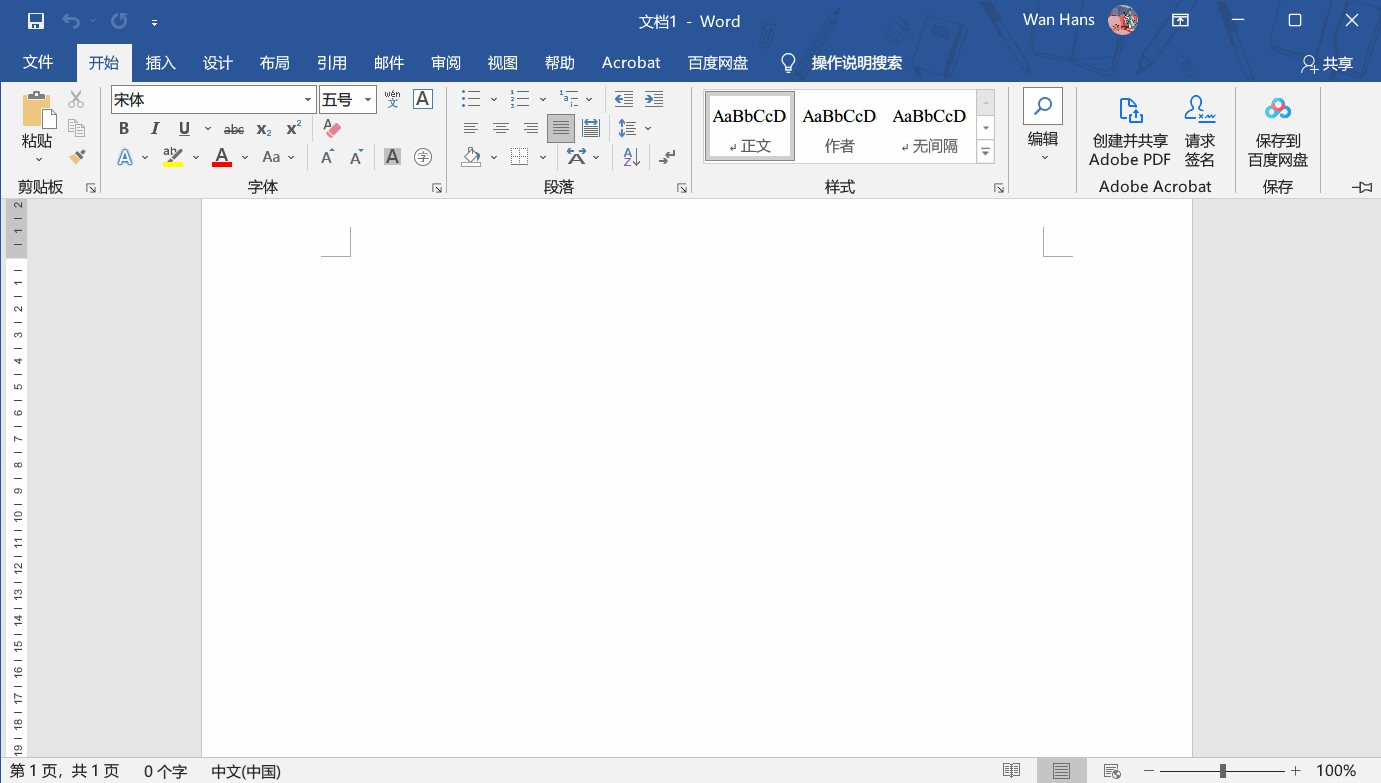
\includegraphics[width=11cm]{assets/Word_2019.jpg}
  \caption{Word 2019 的界面}
  \label{Word_2019}
\end{figure}

近年来,除了这种传统的「年份」Office,微软还推出了一种不断迭代更新的「Office 365」(现改名为「Microsoft 365」)。
Office 365 持续更新,不再使用年份命名,界面上与最新的 Office 版本相一致,功能上随着更新不断增加。
事实上,Office 365 在功能上与最新年份版本的 Office 并无二致,它与年份版本 Office 的最大区别在于各项「云服务」,例如文件跨设备同步等。

\begin{note}
  自 2021 年开始,我国计算机二级考试 Office 科目使用了 Office 2016 作为考试软件。
  如上文所言,Office 2013--2021 乃至 Office 365 的软件界面和操作体验都没有明显的区别,故读者在练习时若实在没有 Office 2016,可以选用其余版本作为替代。
\end{note}

\subsection{Office 的文件格式}

在 Office 2003 及以前版本中,Office 三件套使用的文件格式(扩展名)如表 \ref{Old_Office_File_Format} 所示。
自 Office 2007 开始,微软推出了一套新的 Office 文件格式——「Office 开放 XML 格式」(\href{http://officeopenxml.com/}{Office Open XML},简称「OOXML」)。
这一套格式对应的扩展名如表 \ref{OOXML_File_Format} 所示。

\begin{table}[htb!]
  \begin{minipage}{7.5cm}
    \centering\begin{tabular}{ccc}
      \toprule
      软件 & 扩展名 \\
      \midrule
      Word & \verb|doc| \\
      PPT & \verb|ppt| \\
      Excel & \verb|xls| \\
      \bottomrule
    \end{tabular}
    \caption{曾经的 Office 三件套文件格式}
    \label{Old_Office_File_Format}
  \end{minipage}
  \begin{minipage}{6cm}
    \centering\begin{tabular}{ccc}
      \toprule
      软件 & 扩展名 \\
      \midrule
      Word & \verb|docx| \\
      PPT & \verb|pptx| \\
      Excel & \verb|xlsx| \\
      \bottomrule
    \end{tabular}
    \caption{OOXML 文件格式}
    \label{OOXML_File_Format}
  \end{minipage}
\end{table}

这套新的格式尽管看起来扩展名只是多了个字母「\verb|x|」,但是与旧版格式是\regcolor{完全不兼容}的。
Office 2007 以及之后的各版本,可以打开新旧两种格式的文档,并且在保存文件时可以选择保存为新旧两种格式中的某一种。
下图中,上方「Word 文档 (*.docx)」便是新格式,而下方「Word 97-2003 文档 (*.doc)」则是旧格式。

\begin{figure}[htb!]
  \centering
  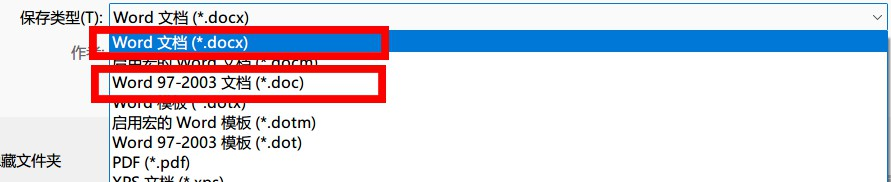
\includegraphics[width=8cm]{assets/Word_formats.jpg}
  \caption{Word 的保存选项}
  \label{Word_Formats}
\end{figure}

新格式(即扩展名带「\verb|x|」的那些格式)相比旧格式支持更多的功能和排版特性。
在今天人们普遍使用 Office 2007 及以上版本的情况下,我们建议始终为自己的文档选用新格式,除非你有明确的理由去选用旧格式(现在的 Office 都是默认保存成新格式的)。

\subsection{Office 的购买和安装}

Office 是付费软件。对于 Office 365,其付费方式是「订阅制」,每年都需要付费才能使用;
对于年份版本的 Office,则采用「买断制」,一次购买便可永久使用。
同一版本的 Office(例如 Office 2019),又根据包含子应用的多少、高级功能的有无、售后服务的等级等,分为不同的档次。
例如「家庭与学生版」只包含 Word、PPT 和 Excel 三件套,没有 VBA 等高级开发功能;
「专业增强版」则包含几乎所有的 Office 功能,但售价高昂。
下图是在微软官网购买 Office 365 的产品介绍页面。

\begin{figure}[htb!]
  \centering
  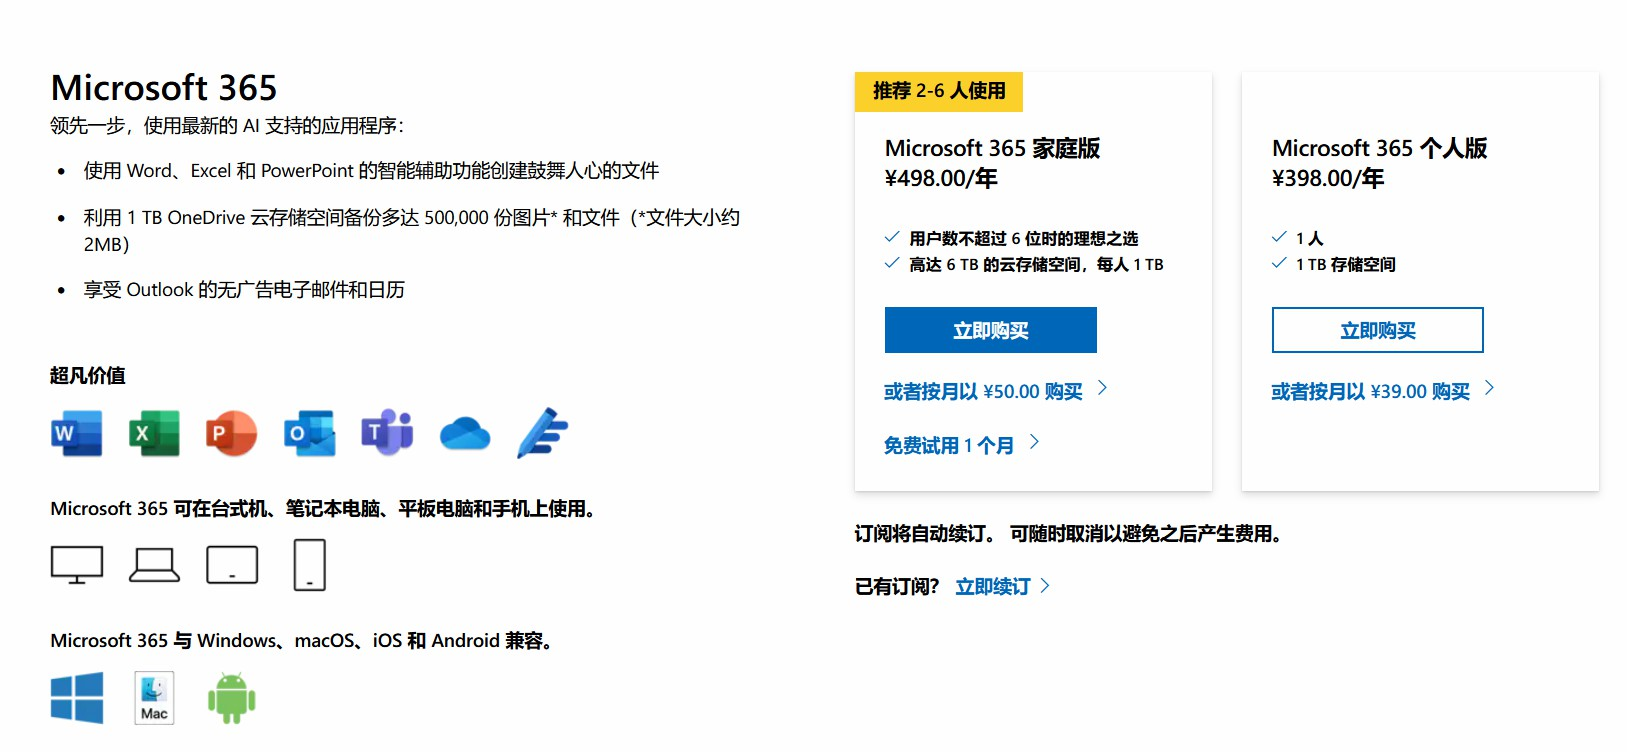
\includegraphics[width=12cm]{assets/Office_365.jpg}
  \caption{Office 365 了解一下}
  \label{Office_365}
\end{figure}

如果需要购买 Office,可以前往\href{https://www.microsoft.com/zh-CN/microsoft-365/buy/microsoft-365}{微软官网}或者 Microsoft Store 进行购买。
如果你是大学生或大学教职工,或许你所在的学校已经为你们批量购买过正版 Office 软件。
此时,你可以通过查阅自己学校官网,或者咨询学校网络信息中心 / 正版软件服务中心来了解正版 Office 的获取方式。
图 \ref{College_Office} 是某学校正版软件平台的截图,在这里可以获取到正版的各版本 Office。

\begin{figure}[htb!]
  \centering
  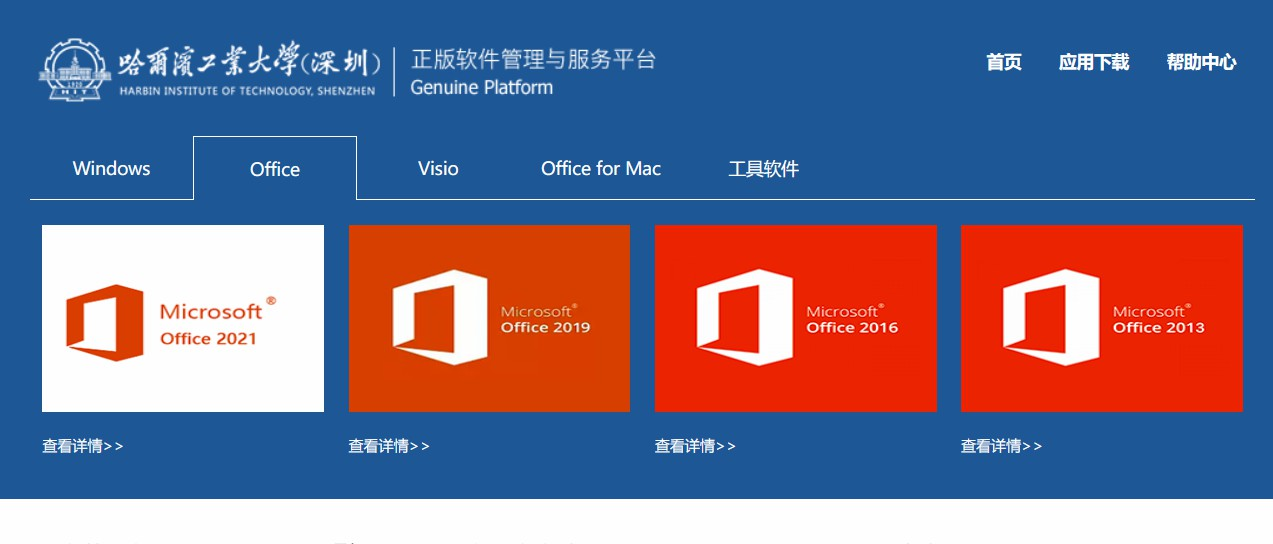
\includegraphics[width=12cm]{assets/College_Office.jpg}
  \caption{某校提供的 Office}
  \label{College_Office}
\end{figure}

今天,许多笔记本电脑和品牌机台式机在出厂时会附赠用户一套正版 Office 软件。
这种情况下,机器首次开机后内置的 Office 软件(例如 Word 和 PPT)都是可以直接使用的。
我们只需要按照软件的提示,登录或创建一个自己的微软账号,即可完成正版验证。
不过,如果你是在电脑城组装的电脑,或者使用的非品牌零售渠道的机器,那么很可能没有这项福利。
图 \ref{JD_Office_Gift} 是在京东平台购买某笔记本电脑时的 Office 附赠提示。

\begin{figure}[htb!]
  \centering
  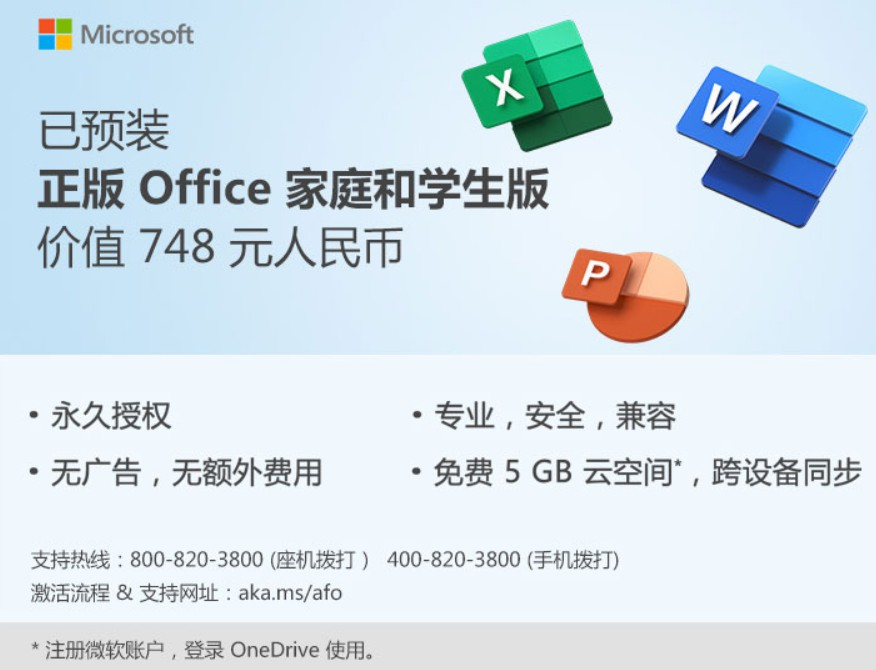
\includegraphics[width=7.5cm]{assets/JD_Office_Gift.jpg}
  \caption{买电脑送 Office}
  \label{JD_Office_Gift}
\end{figure}

Office 软件的安装方式比较简单。
取决于你获取到软件的方式,如果你是通过 Microsoft Store 购买的 Office,那么直接在 Microsoft Store 点击「安装」就可以完成 Office 软件的安装。
对于通过其他官方途径获取的 Office 安装器,大多数情况下也只需要简单地双击并按提示操作即可完成安装。

Office 这种软件自然免不了被盗版的命运。
需要注意的是,在互联网上有很多民间二次打包的「破解版」Office,这种 Office 直接安装后无需更多操作就能免费使用。
我们不建议大家使用这样的 Office——除了「盗版」本身不值得提倡外,这些二次打包的 Office 往往经过一些「精简」或者「魔改」,这可能导致少数情况下软件工作不正常甚至无法使用。
此外,这些魔改 Office 往往会有一些使用上的不便,例如每次启动时触发 UAC 弹窗(弹出窗口「你要允许此应用……」),以及文件关联莫名失效等。

\subsection{「网页版」 Office}

即使你没有购买和安装过 Office,你或许仍会发现电脑的「开始菜单」中有 Office 甚至 Word、PPT、Excel 等软件的图标,例如:

\begin{figure}[htb!]
  \centering
  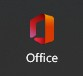
\includegraphics[width=3cm]{assets/Office_Web_Icon.jpg}
  \caption{网页版Office的图标}
  \label{Office_Web_Icon}
\end{figure}

如果你尝试去点击这些 app,会发现打开了一个网页。
在这个页面按提示登录微软账号,最后会来到这个页面:

\begin{figure}[htb!]
  \centering
  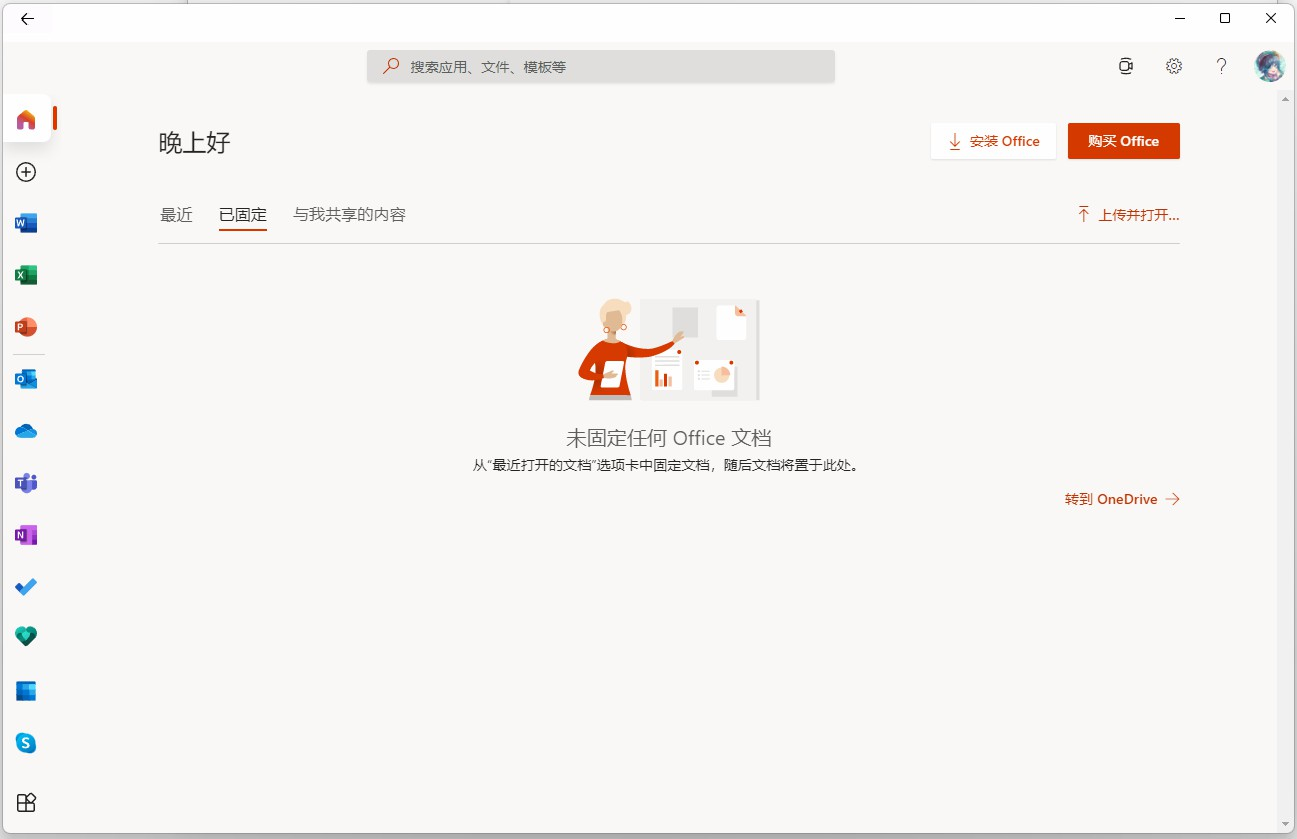
\includegraphics[width=10cm]{assets/Office_Web.jpg}
  \caption{网页版Office的界面}
  \label{Office_Web}
\end{figure}

这是微软提供的免费的「网页版」Office,类似于腾讯文档或金山文档等网页产品。
点击左侧的 Word、Excel 等图标,会打开对应的网页版应用。
这些网页版的 Office 可以免费使用,但功能受限,且只有在网络良好时才能正常工作,故只能作为没有安装 Office 的应急替代品。

这个「网页版」Office 本质就是几个链接,没有软件的本体,是可以卸载的。
卸载方式可参见\nameref{basic-maintenance}。

\subsection{选择 Office 的原因}

在今天,Office 文件格式(即「\verb|doc|」、「\verb|pptx|」等文件格式)在人们的日常工作中有着绝对无可动摇的地位——绝大多数的工作资料都是通过这套格式的文件进行交换的。
Office 作为推出这套格式的本家,自然与这套格式最为契合。
因此,\regcolor{选择 Office 的最主要原因,便是它对 Office 文件格式的无缝支持}。
WPS 尽管对这套格式也有着相当高的支持度,但在少数情况下,仍然会出现排版错乱、内容丢失等情况。
至于其他办公软件,大多对于 Office 文件格式的支持只能说「勉强」。

选择 Office 的另一个原因是,\regcolor{Office 作为微软自家出品的软件,在 Windows 操作系统上具有相对出色的性能表现和操作体验。}
在一众办公软件中,Office 的操作手感比较舒适,且与 WPS 相比,Office 界面简洁、没有繁杂的广告和其他多余功能。
下图是在 Windows 11 系统上,Office 三件套软件的界面。

\begin{figure}[htb!]
  \centering
  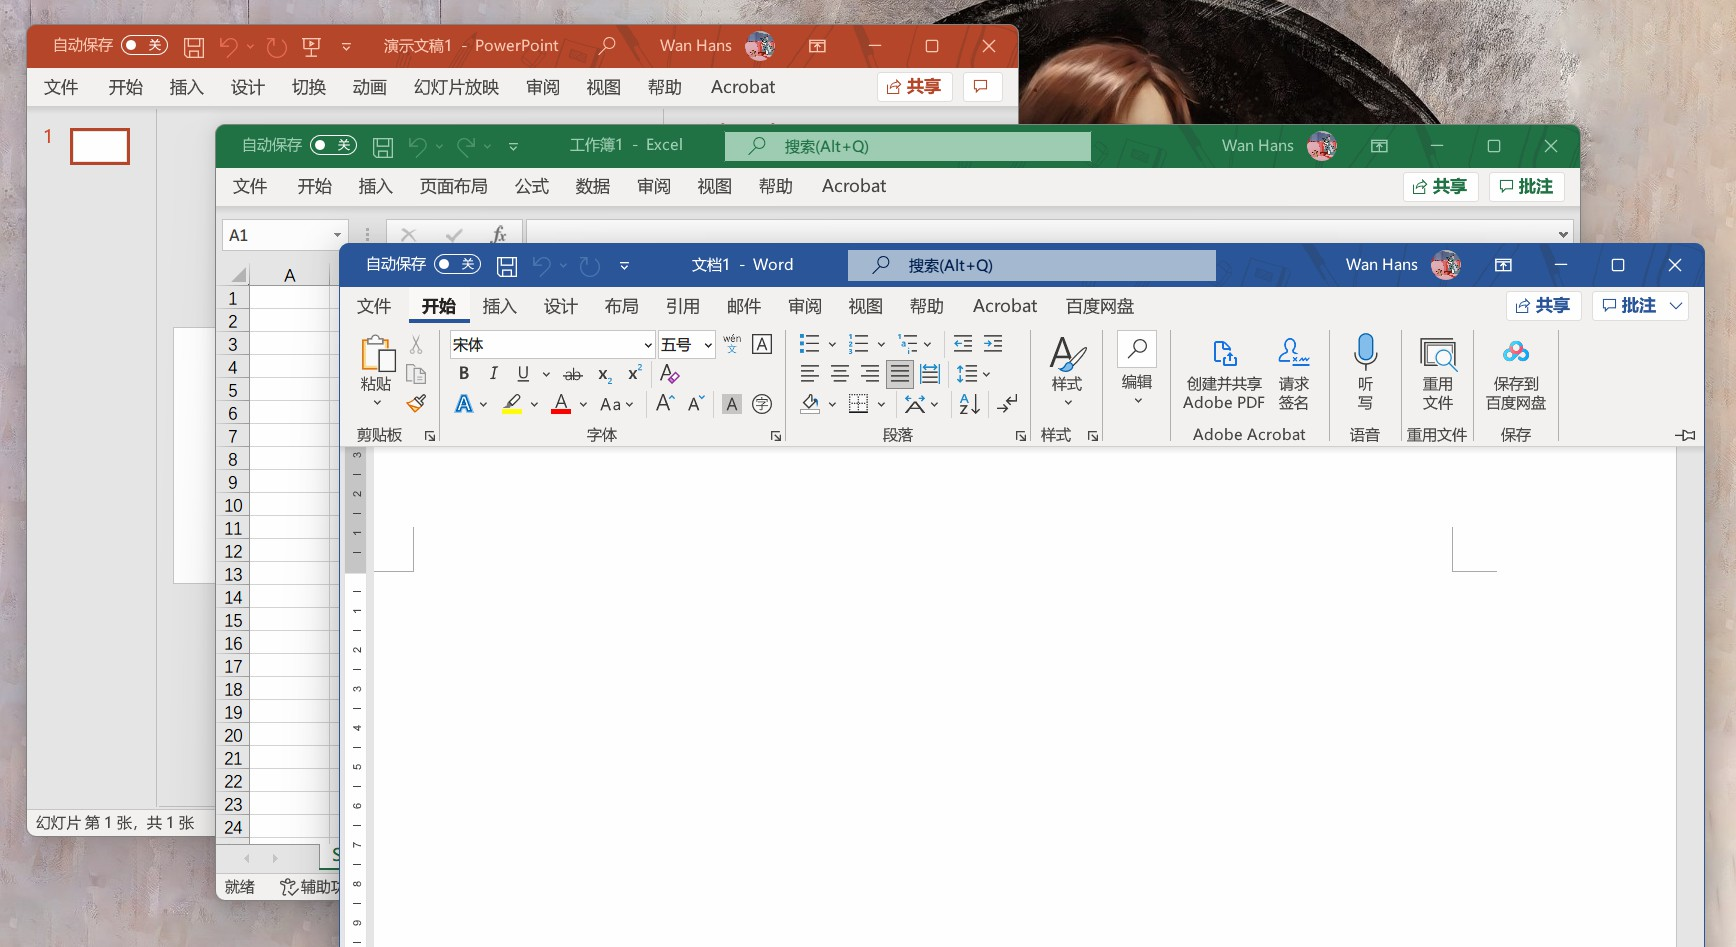
\includegraphics[width=11cm]{assets/Office_on_Win_11.jpg}
  \caption{Windows 11 上的 Office}
  \label{Office_on_Win_11}
\end{figure}

\section{WPS}

\regcolor{WPS 是除了 Office 自身外,对 Office 文件格式(包含新旧两种格式)支持最好的办公软件},可以说没有之一。
WPS 包含三个主要的子组件,分别是「WPS 文字」「WPS 演示」和「WPS 表格」,依次对标 Office 套装中的 Word、PPT 和 Excel。
WPS 使用类似于 Office 的界面,默认使用 Office 文件格式进行文件保存,因而在大多数情况下都可以作为 Office 的替代品。

\subsection{WPS 的历史}

WPS 是由\href{https://www.kingsoft.com/}{金山公司}开发的国产免费软件。
WPS 的历史最早可以追溯到 1985 年,与很多人的臆想不同,WPS 并不是靠「模仿」Office 起家的。
在那时,微软的 Office 还没有支持中文,而 WPS 作为一套独立的中文文字处理系统(word processing system, WPS),在中国市场上占有很大一席之地。
1994 年,微软的 Office 开始进入中国市场。
为了和 WPS 竞争市场,微软和金山达成协议,双方能够交叉使用对方的文件格式——这是 WPS 得以完整支持 Office 文件格式的原因。
后来,WPS 逐渐失去市场优势,于是开始走上模仿 Office 的道路,从原来的单一「文字处理系统」变成了和 Office 相仿的办公软件套装,并在操作界面上有意地向 Office 靠拢。
今天的 WPS 在办公软件的基础上,又加入了「协作办公」「云服务」等许多增值服务,建立了一整套自己的办公解决方案。

\subsection{WPS 的使用}

今天 WPS 的界面与近年新版 Office 软件的界面高度相似。
下图是 WPS 文字 2019 版本的界面截图。
对于大多数 Office 软件中的操作,WPS 中的操作方式都是相同或近似的。

\begin{figure}[htb!]
  \centering
  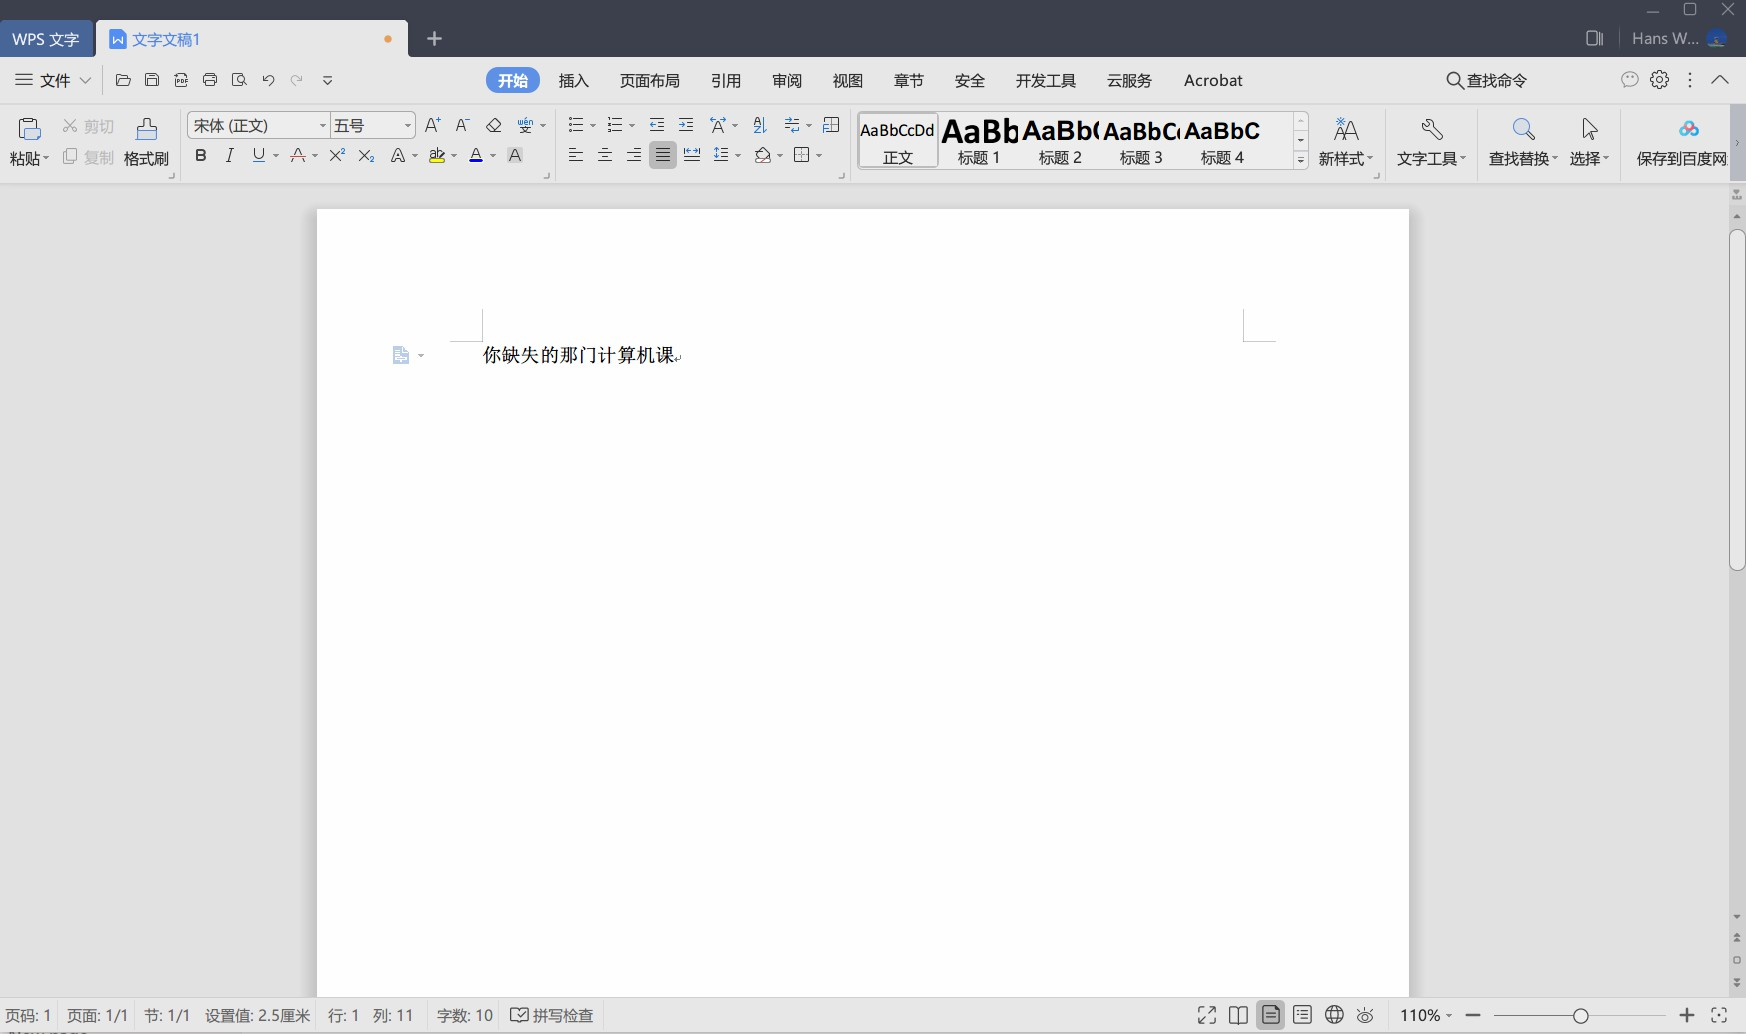
\includegraphics[width=10cm]{assets/WPS.jpg}
  \caption{WPS 文字 2019 的界面}
  \label{WPS}
\end{figure}

\subsection{选择 WPS 的理由}

WPS 对 Office 文件格式有着高度的兼容性,这意味着在绝大多数情况下 WPS 都可以作为 Office 软件的替代品。
同时,WPS 是免费软件。
这意味着,你可以在没有任何额外成本的情况下合理合法地使用它,同时获得对 Office 文件格式的最大兼容度并保持 Office 的使用习惯。

WPS 针对中国用户的使用习惯推出了一系列额外功能。
WPS 有自己的模板库,称为「稻壳儿」。
在稻壳儿中,你能找到各种各样的适合不同场景的文稿、幻灯片和表格模板,并将它们应用在自己的文档之中(可能需要额外付费)。
在一些情况下,使用这些模板能够省时省力地制作出精美的文档。
又比如,WPS 提供了自己的云服务平台(金山文档),借助金山文档能够实现多人协同编辑文件等高级功能。
下图是「稻壳儿」中提供的部分模板。

\begin{figure}[htb!]
  \centering
  
\includegraphics[width=11cm]{assets/WPS_Template.jpg}
  \caption{「稻壳儿」模板}
  \label{WPS_Template}
\end{figure}

\practice

\begin{enumerate}
  \item 你电脑上安装有 Office 吗?你能熟练地使用它们吗?你知道你所使用的 Office 软件的版本吗?
  \item 你有使用 WPS 吗?如果有,试试探索「稻壳儿」模板商城。
  \item 前往电商平台查看一些笔记本电脑的商品详情,看看它们是否有将正版 Office 软件一并附赠。
\end{enumerate}